\documentclass[12pt,a4paper]{article}
\usepackage{geometry}
\geometry{left=2.5cm,right=2.5cm,top=2.0cm,bottom=2.5cm}
\usepackage[english]{babel}
\usepackage{amsmath,amsthm}
\usepackage{amsfonts}
\usepackage{bm}
\usepackage[longend,ruled,linesnumbered]{algorithm2e}
\usepackage{siunitx}
\usepackage{fancyhdr}
\usepackage{ctex}
\usepackage{array}
\usepackage{listings}
\usepackage{color}
\usepackage{graphicx}
\usepackage{float}
\usepackage{caption}
\usepackage{longtable}
\begin{document}
    \title{\heiti{《机器学习》课程第 {$2$} 次作业}}
    \date{}
    \author{姓名:\underline{刘哲}~~~~~~学号:\underline{2022103691}~~~~~~}
    \maketitle
    \section{\heiti{钓鱼问题}}
    \vspace{10pt}
    \subsubsection*{A}
    训练数据模型1的P-R图和RUC曲线图:
    \begin{figure}[H]
        \centering
        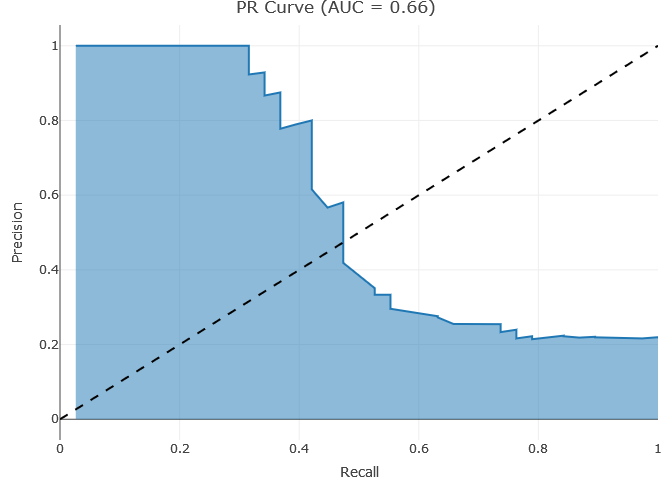
\includegraphics[scale=0.65]{TrainPR1.png}
    \end{figure}
    \begin{figure}[H]
        \centering
        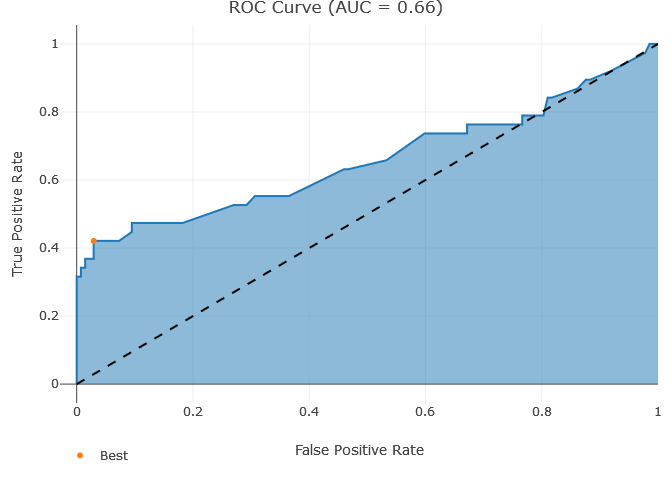
\includegraphics[scale=0.65]{TrainROC1.png}
    \end{figure}
    训练数据模型2的P-R图和RUC曲线图:
    \begin{figure}[H]
        \centering
        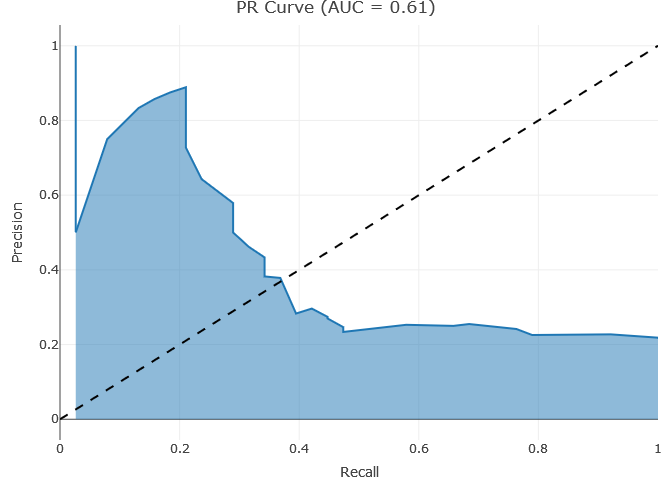
\includegraphics[scale=0.65]{TrainPR2.png}
    \end{figure}
    \begin{figure}[H]
        \centering
        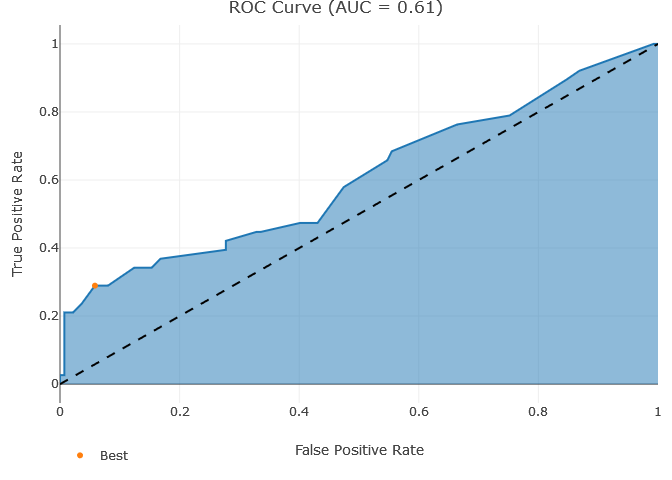
\includegraphics[scale=0.65]{TrainROC2.png}
    \end{figure}
    测试数据模型1的P-R图和RUC曲线图:
    \begin{figure}[H]
        \centering
        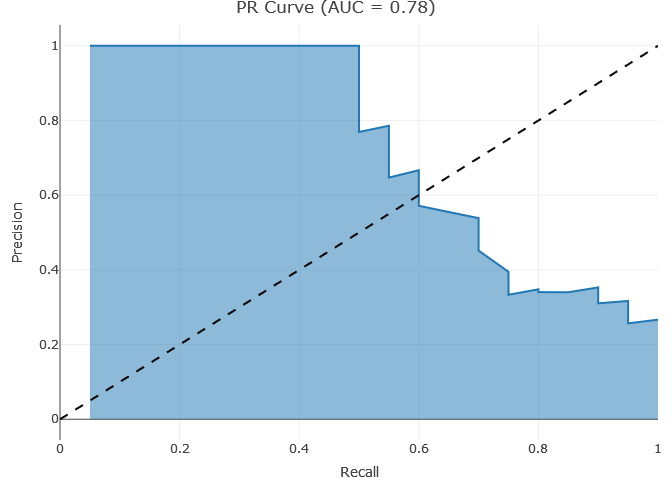
\includegraphics[scale=0.65]{TestPR1.png}
    \end{figure}
    \begin{figure}[H]
        \centering
        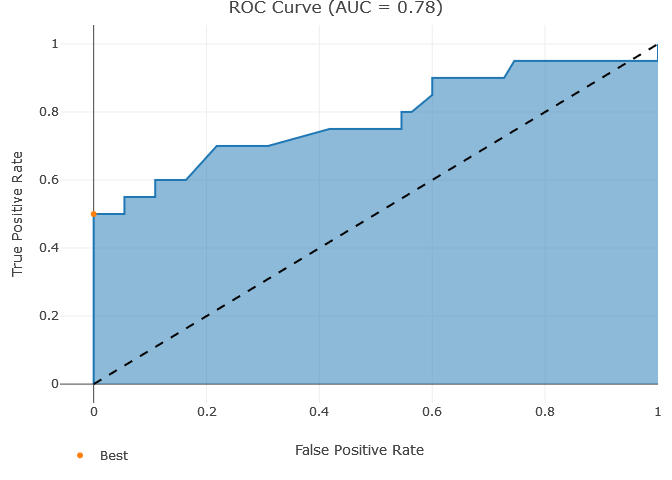
\includegraphics[scale=0.65]{TestROC1.png}
    \end{figure}
    测试数据模型2的P-R图和RUC曲线图:
    \begin{figure}[H]
        \centering
        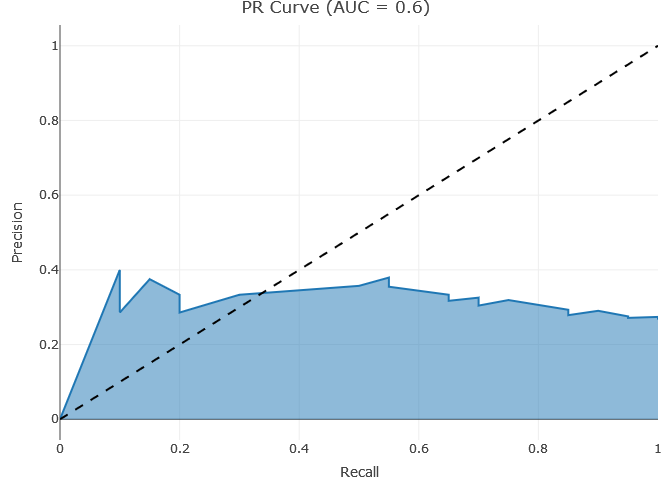
\includegraphics[scale=0.65]{TestPR2.png}
    \end{figure}
    \begin{figure}[H]
        \centering
        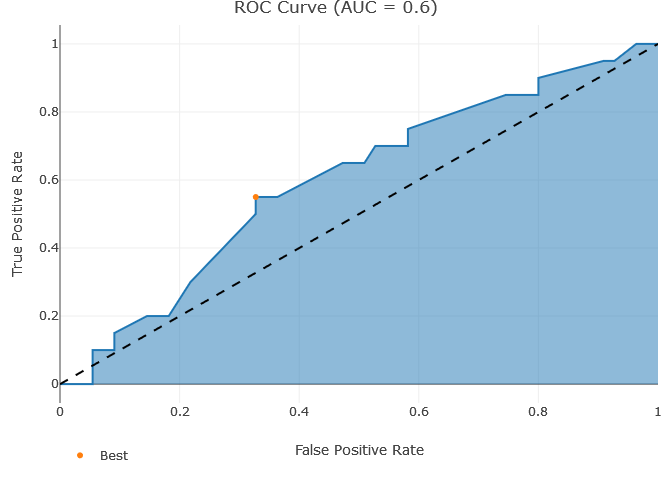
\includegraphics[scale=0.65]{TestROC2.png}
    \end{figure}
    各个模型的AUC如图所示,因为模型1在测试数据上具有最高的AUC=0.78,所以认为模型1的整体预测效果最佳。\par
    选取预测阈值依据的是Youden指数:
    \begin{equation}
        Youden's\ Index = sensitivity + specificity - 1
    \end{equation}
    Youden指数最大的点,即为最佳阈值点。由此可知,模型1的最佳阈值为3.3354,模型2的最佳阈值为1.13828。
    \subsubsection*{B}
    根据A中给出的各模型的阈值,计算模型1的混淆矩阵为
    \begin{longtable}{|c|c|c|}
        \hline
         & Truth 0 & Truth 1\\
        \hline
        Prediction 0 & 133 & 22\\
        \hline
        Prediction 1 & 4 & 16\\
        \hline
    \end{longtable}
    模型2的混淆矩阵为
    \begin{longtable}{|c|c|c|}
        \hline
         & Truth 0 & Truth 1\\
        \hline
        Prediction 0 & 129 & 27\\
        \hline
        Prediction 1 & 8 & 11\\
        \hline
    \end{longtable}
    \section{\heiti{似然比方法}}
    \vspace{10pt}
    论文主要介绍了特征变量型似然比和评分法似然比两种似然比的计算方法。
    假设有两组数据$\bm{y}_1$和$\bm{y}_2$,要检验它们是否属于同一个的数据源,提出假设检验如下:
    \begin{equation}
        H_p: \bm{y}_1\text{和}\bm{y}_2\text{同源}\ vs\ H_d: \bm{y}_1\text{和}\bm{y}_2\text{不同源}
    \end{equation}\par
    首先,假设背景数据$\bm{x}$不变,特征变量型似然比的计算公式为
    \begin{equation}
        LR = \frac{f\left(\bar{\bm{y}_1},\bar{\bm{y}_2}|\bm{U},\bm{C},\bar{\bm{x}},H_p\right)}{f\left(\bar{\bm{y}_1},\bar{\bm{y}_2}|\bm{U},\bm{C},\bar{\bm{x}},H_d\right)}
    \end{equation}
    如果两组数据$\bm{y}_1$和$\bm{y}_2$同源,则它们的均值之差$(\bar{\bm{y}_1}-\bar{\bm{y}_2})$应该服从正态分布,且它们对背景数据$\bm{x}$具有相同的影响,即
    \begin{equation}
        \begin{split}
            f&\left(\bar{\bm{y}_1},\bar{\bm{y}_2}|\bm{U},\bm{C},\bar{\bm{x}},H_p\right)=f\left(\bar{\bm{y}_1}-\bar{\bm{y}_2},\bar{\bm{y}}|\bm{U},\bm{C},\bar{\bm{x}},H_p\right)\\
                &=\left(2\pi\right)^{-p}\left|\frac{\bm{U}}{n_1}+\frac{\bm{U}}{n_2}\right|^{-\frac{1}{2}}\exp\left\{-\frac{1}{2}\left(\bar{\bm{y}_1}-\bar{\bm{y}_2}\right)^T\left(\frac{\bm{U}}{n_1}+\frac{\bm{U}}{n_2}\right)^{-1}\left(\bar{\bm{y}_1}-\bar{\bm{y}_2}\right)\right\}\\
                &\times\left|\frac{\bm{U}}{n_1+n_2}+\bm{C}\right|^{-\frac{1}{2}}\exp\left\{-\frac{1}{2}\left(\bar{\bm{y}}-\bar{\bm{x}}\right)^T\left(\frac{\bm{U}}{n_1+n_2}+\bm{C}\right)^{-1}\left(\bar{\bm{y}}-\bar{\bm{x}}\right)\right\}
        \end{split}
    \end{equation}
    如果两组数据$\bm{y}_1$和$\bm{y}_2$不同源,则它们的均值之间相互独立,且它们各自独立对背景数据$\bm{x}$产生影响,即
    \begin{equation}
        \begin{split}
            f&\left\{\bar{\bm{y}_1},\bar{\bm{y}_2}|\bm{U},\bm{C},\bar{\bm{x}},H_d\right\}=f\left(\bar{\bm{y}_1}|\bm{U},\bm{C},\bar{\bm{x}},H_d\right)f\left(\bar{\bm{y}_2}|\bm{U},\bm{C},\bar{\bm{x}},H_d\right)\\
                &=\left(2\pi\right)^{-p}\left|\frac{\bm{U}}{n_1}+\bm{C}\right|^{-\frac{1}{2}}\exp\left\{-\frac{1}{2}\left(\bar{\bm{y}_1}-\bar{\bm{x}}\right)^T\left(\frac{\bm{U}}{n_1}+\bm{C}\right)^{-1}\left(\bar{\bm{y}_1}-\bar{\bm{x}}\right)\right\}\\
                &\times\left|\frac{\bm{U}}{n_2}+\bm{C}\right|^{-\frac{1}{2}}\exp\left\{-\frac{1}{2}\left(\bar{\bm{y}_2}-\bar{\bm{x}}\right)^T\left(\frac{\bm{U}}{n_2}+\bm{C}\right)^{-1}\left(\bar{\bm{y}_2}-\bar{\bm{x}}\right)\right\}
        \end{split}
    \end{equation}
    其中$\bm{y}$、$\bm{y}_1$、$\bm{y}_2$和$\bm{x}$均服从正态假设,且$\bm{y}$、$\bm{y}_1$和$\bm{y}_2$同方差。
    $\bm{U}$表示类内协方差矩阵,$\bm{C}$表示类间协方差矩阵,由背景数据$\bm{x}$获得其估计,计算公式为
    \begin{gather}
        \hat{\bm{U}}=\frac{\bm{S}_w}{m\left(n-1\right)}\\
        \hat{\bm{C}}=\frac{\bm{S}^*}{m-1}-\frac{\bm{S}_w}{nm\left(n-1\right)}\label{c}
    \end{gather}
    其中,$\bm{S}_w=\sum_{i=1}^m\sum_{j=1}^n\left(x_{ij}-\bar{x}_i\right)\left(x_{ij}-\bar{x}_i\right)^T$,$\bm{S}^*=\sum_{i=1}^m\left(x_i-\bar{x}\right)\left(x_i-\bar{x}\right)^T$,$m$为类的个数,$n$为样本中每个类的样品数。
    特征变量型似然比方法以两种不同的前提假设分别计算了联合密度函数,将它们的比值作为似然比统计量。\par
    其次,评分法似然比的计算公式为
    \begin{equation}
        \hat{SLR}=\frac{f\left(s_p|H_p,I\right)}{f\left(s_d|H_d,I\right)}
    \end{equation}
    其中$s_p$表示同源比对分数(组内),$s_d$表示非同源比对分数(组间),$I$为背景信息。
    在分数为连续型变量时,$f$表示概率密度函数;在分数为离散型变量时,$f$表示概率分布函数。
    对分数的分布进行非参数检验,如果分布为参数分布,可以使用其概率函数的比值作为似然比;如果分布不符合常见的参数分布,则使用合适的非参数分布计算似然比。
    评分法似然比方法建立了一个评分体系,在这个评分体系下给出数据同源或不同源的比对分数,进而形成两个分数的分布,代表两种假设成立的可能性,使用分数分布的比值作为似然比统计量。\par
    对于似然比检验来说,如果似然比大于一个不小于$1$的阈值,认为同源假设下的似然函数显著大于不同源假设下的似然函数,则两组数据同源或相关的可能性较大;
    如果似然比小于一个不大于$1$的阈值,认为不同源假设下的似然函数显著大于同源假设下的似然函数,则两组数据不同源且相互独立的可能性较大。\par
    研究人员常使用直方图、Tippett图、DET图和ECE图来评价似然比的计算结果,评价指标为识别力和区分力。
    其中,识别力反映似然比模型区分两种假设对应的似然比数值的能力,区分力反映似然比模型在支持某一假设时的正确程度。
    直方图是将支持两种假设的对数似然比数值分布以直方图的形式在数轴上表示出来,两组直方在数轴上的重叠程度越小,似然比模型的识别能力越强。
    Tippett图是支持两组假设的对数似然比数值的累积分布图,两条累积分布曲线在垂直方向上的分离程度越大,似然比模型的识别能力越强。
    DET图展示的是似然比模型的假阳性率与假阴性率之间的相互关系,曲线越靠近坐标轴零点位置,似然比模型的识别能力越强。
    ECE图是通过设置罚函数,结合PAV(Pool Adjacent Violators)算法绘制的图形,它是唯一一个能同时反映似然比模型识别力(discrimination)和区分力(calibration)的图形,
    经过PAV算法的似然比数值曲线越靠近横轴识别力越强,且真实似然比数值曲线与经过PAV算法的似然比数值曲线的距离越小区分力越强。
    \section{\heiti{计算似然比}}
    \vspace{10pt}
    计算似然比的函数见代码。\par
    在计算时发现,公式(\ref{c})可能会导致$\hat{\bm{C}}$非正定,这使得似然比计算公式中的部分行列式为负值,无法求其$-1/2$次方。
    因此,暂且将行列式取绝对值,得到墨迹鉴定数据的似然比如下:
    \begin{longtable}{c|c|c|c|c|c}
        \hline
        Object & 1 & 2 & 3 & 4 & 5\\
        \hline
        LR & \num{5.359e-11} & \num{2.897e-08} & \num{1.154e+02} & \num{4.744e-20} & \num{3.316e-09}\\
        \hline
    \end{longtable}
\end{document}